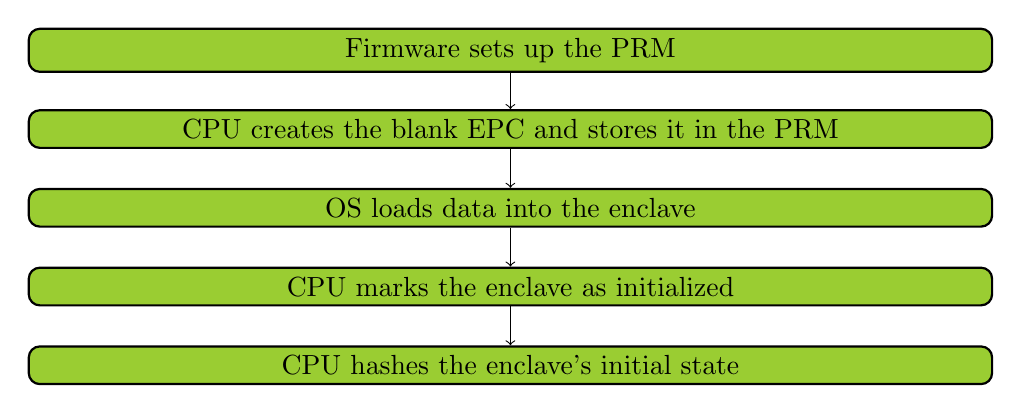
\begin{tikzpicture}[
    block/.style ={rectangle, draw=black, thick, fill=YellowGreen,
          text width=12cm, text centered, rounded corners},
    line/.style ={draw, ->}
]

\node[block] (s1) at (0,0) {Firmware sets up the PRM};
\node[block, below of = s1] (s3) {CPU creates the blank EPC and stores it in the PRM};
\node[block, below of = s3] (s5) {OS loads data into the enclave};
\node[block, below of = s5] (s10) {CPU marks the enclave as initialized};
\node[block, below of = s10] (s15) {CPU hashes the enclave’s initial state};

\path [line] (s1) -- (s3);
\path [line] (s3) -- (s5);
\path [line] (s5) -- (s10);
\path [line] (s10) -- (s15);

\end{tikzpicture}
